\documentclass[tikz, margin=2mm]{standalone}
\usepackage{tikz}
\usetikzlibrary{arrows.meta,backgrounds,matrix}

\begin{document}
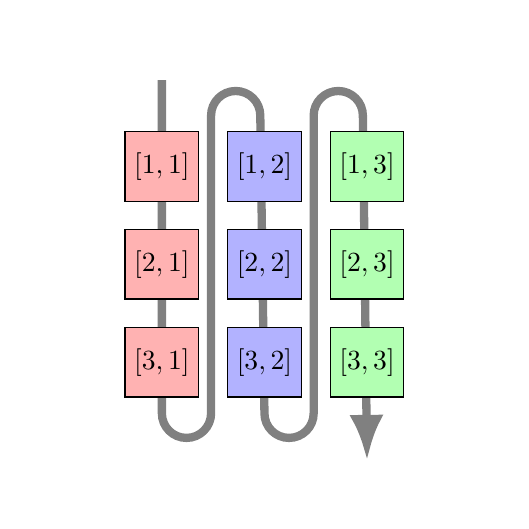
\begin{tikzpicture}[%
    arraynode/.style={
        draw,
        rectangle, 
        minimum size = 25,
        node contents={[\the\numexpr\pgfmatrixcurrentrow\relax,
                        \the\numexpr\pgfmatrixcurrentcolumn\relax]},
        alias=n\the\numexpr\pgfmatrixcurrentrow\relax\the\numexpr\pgfmatrixcurrentcolumn\relax
        },
    array/.style={%
        matrix of math nodes,
        nodes = arraynode,
        column sep = 10,
        row sep = 10,
        nodes in empty cells,
        column 1/.style={nodes={fill=red!30}},
        column 2/.style={nodes={fill=blue!30}},
        column 3/.style={nodes={fill=green!30}}}, 
]

\draw[white] (-3,-3) rectangle (+3,+3);

\matrix[array] {
&&\\
&&\\
&&\\
};

\begin{scope}[on background layer]
\draw[-{LaTeX}, line width=3pt, black!50] ([yshift=6.5mm]n11.north) 
        foreach \i [count=\ni from 1] in {1,...,2}{
           -- ([yshift=-2mm]n3\i.south) arc(180:360:3.125mm)
           -- ([shift={(6.25mm,2mm)}]n1\i.north) arc(180:0:3.125mm)}
           -- ([yshift=-8mm]n33.south);
\end{scope}
\end{tikzpicture}%
\end{document}